\section{Resoconto delle Attività di Verifica}
\subsection{Macrofase RTB}
\subsubsection{M14IG - Indice di Gulpease}
\begin{figure}[H]
    \centering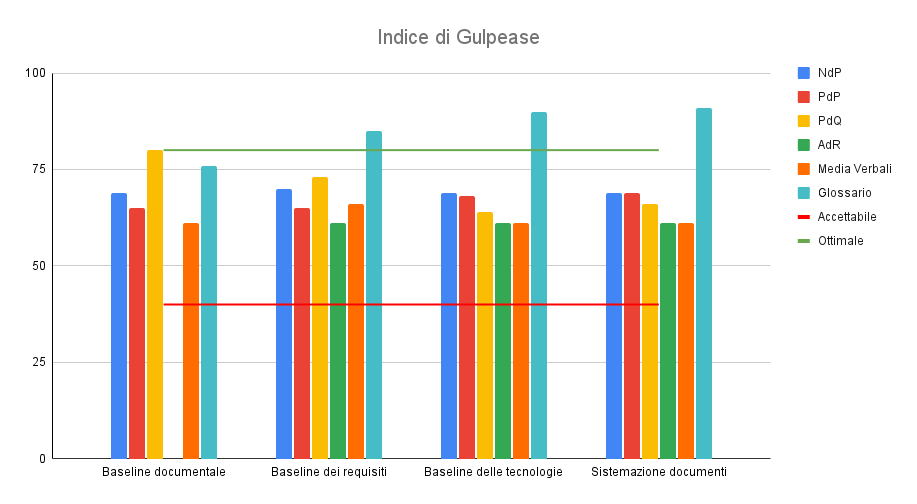
\includegraphics[width=0.8\textwidth, height=0.8\textheight,keepaspectratio]{images/RTB-Indice-di-Gulpease.png}
    \caption{Grafico dell'indice di Gulpease dei documenti nelle varie fasi dell'RTB.}
\end{figure}    

\subsubsection{M15VC - Variazione di Costo}
\begin{figure}[H]
    \centering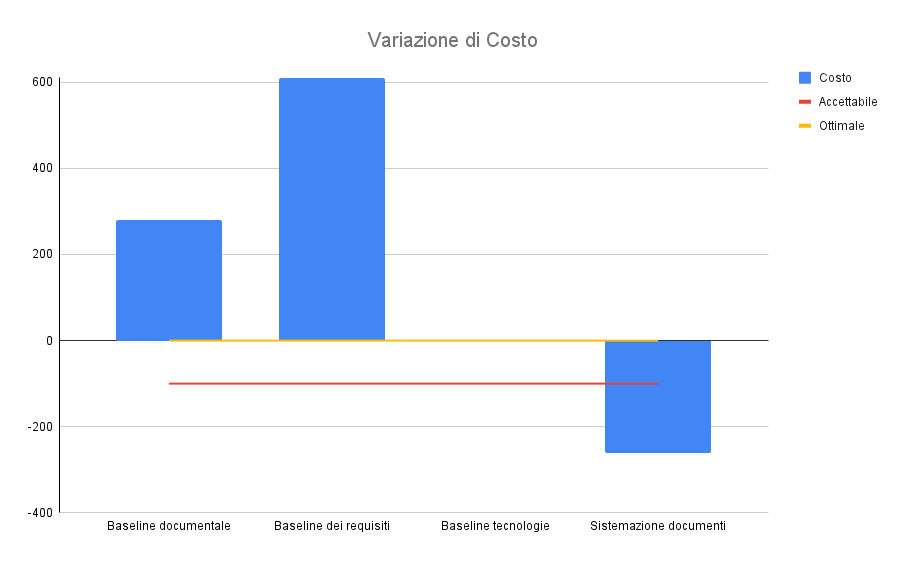
\includegraphics[width=0.8\textwidth, height=0.8\textheight,keepaspectratio]{images/RTB-Variazione-di-Costo.png}
    \caption{Grafico che indica come sono variati i costi rispetto a quelli preventivati nelle varie fasi dell'RTB.}
\end{figure}    

\subsubsection{M16VP - Variazione di Piano}
\begin{figure}[H]
    \centering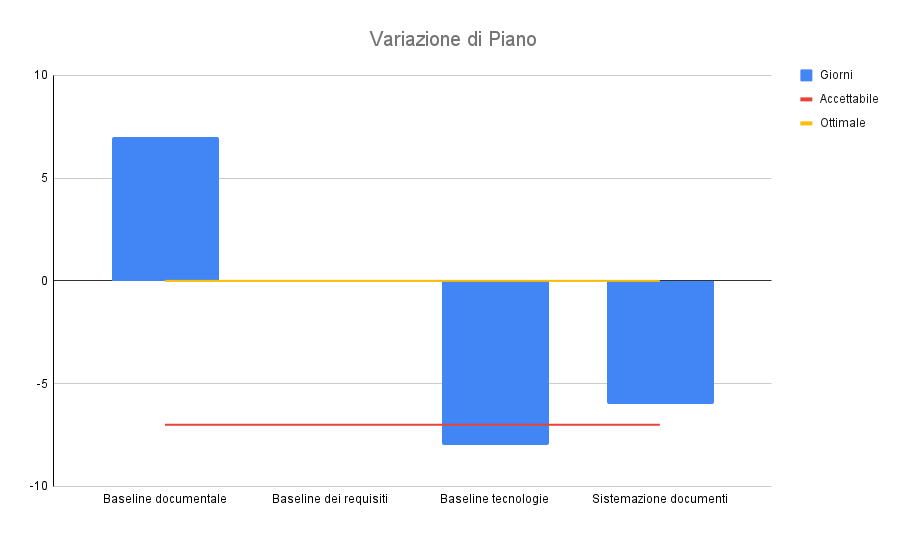
\includegraphics[width=0.8\textwidth, height=0.8\textheight,keepaspectratio]{images/RTB-Variazione-di-Piano.png}
    \caption{Grafico che indica come è variata la pianficazione rispetto al preventivo nelle varie fasi dell'RTB.}
\end{figure}  


\subsection{Macrofase PB}
\subsubsection{M14IG - Indice di Gulpease}
\begin{figure}[H]
    \centering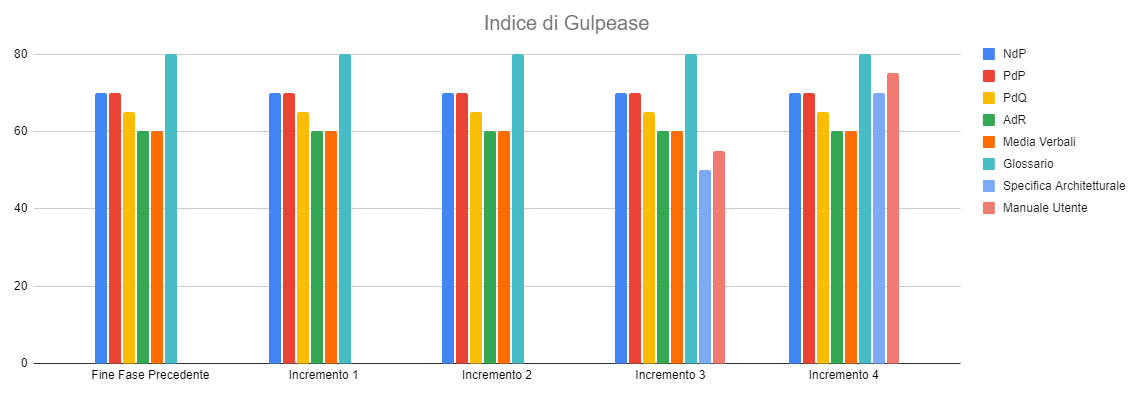
\includegraphics[width=\textwidth, height=\textheight,keepaspectratio]{images/PB-Indice-di-Gulpease.png}
    \caption{Grafico dell'indice di Gulpease dei documenti nelle varie fasi della PB.}
\end{figure}    

\subsubsection{M15VC - Variazione di Costo}
\begin{figure}[H]
    \centering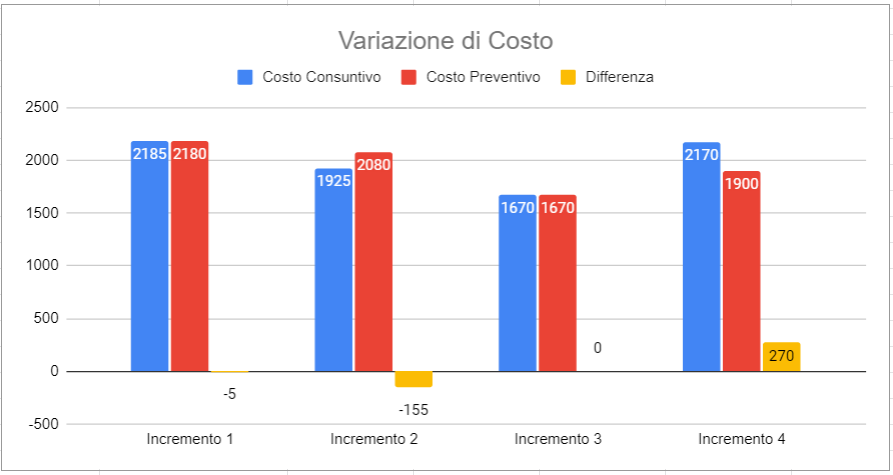
\includegraphics[width=0.8\textwidth, height=0.8\textheight,keepaspectratio]{images/PB-Variazione-di-Costo-2.png}
    \caption{Grafico che indica come sono variati i costi rispetto a quelli preventivati nelle varie fasi della PB.}
\end{figure}    

\subsubsection{M16VP - Variazione di Piano}
\begin{figure}[H]
    \centering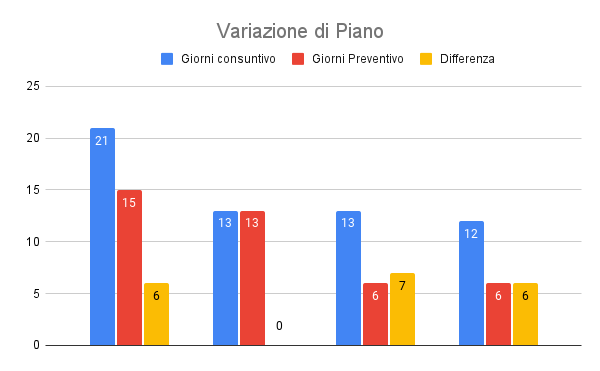
\includegraphics[width=0.8\textwidth, height=0.8\textheight,keepaspectratio]{images/PB-Variazione-di-Piano-3.png}
    \caption{Grafico che indica come è variata la pianificazione rispetto al preventivo nelle varie fasi della PB.}
\end{figure}  

\subsubsection{M8CC - Code Coverage}
\begin{figure}[H]
    \centering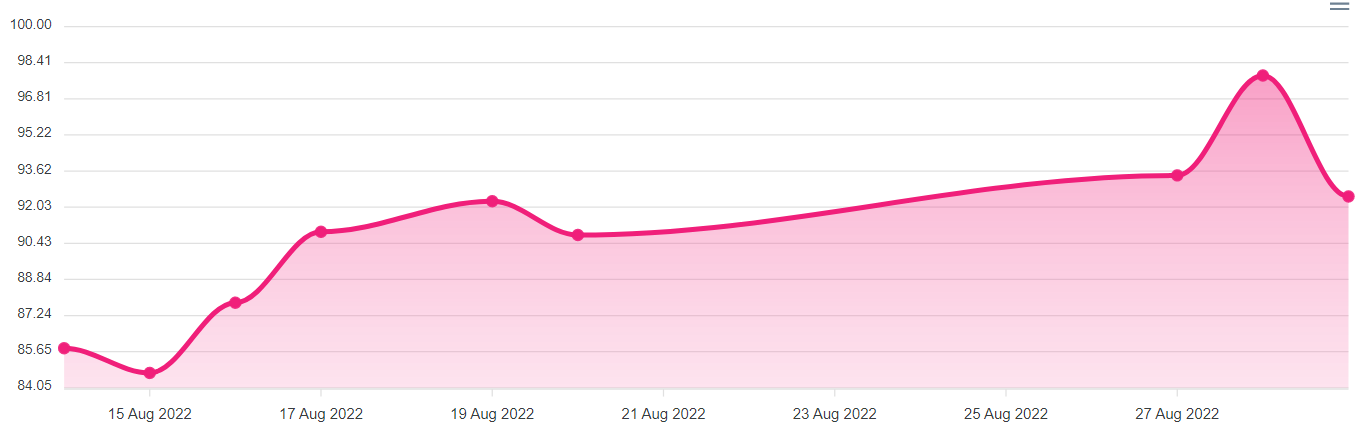
\includegraphics[width=0.8\textwidth, height=0.8\textheight,keepaspectratio]{images/PB-Code-Coverage.png}
    \caption{Grafico che indica come è variata la percentuale di codice coperto da Test nel corso del progetto.}
\end{figure}  

\subsubsection{M1PRR - Percentuale di Requisiti Obbligatori Soddisfatti}
\begin{figure}[H]
    \centering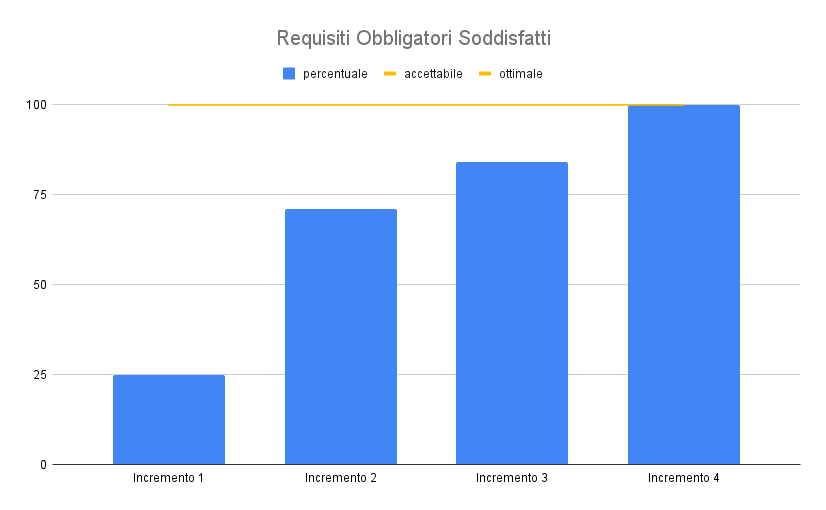
\includegraphics[width=0.8\textwidth, height=0.8\textheight,keepaspectratio]{images/PB-Requisiti-Obbligatori-Soddisfatti.png}
    \caption{Grafico che indica come è variata la percentuale di requisiti obbligatori soddisfatti.}
\end{figure}  

\subsubsection{M2PDR - Percentuale di Requisiti Desiderabili Soddisfatti}
\begin{figure}[H]
    \centering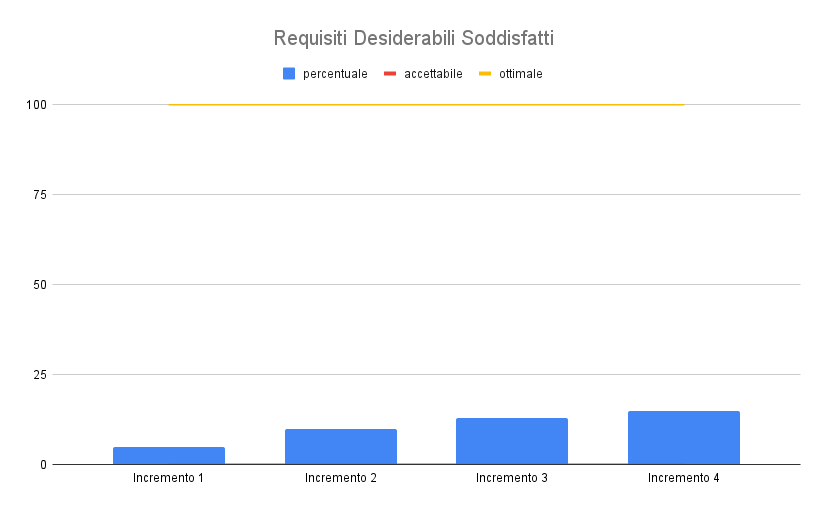
\includegraphics[width=0.8\textwidth, height=0.8\textheight,keepaspectratio]{images/PB-Requisiti-Desiderabili-Soddisfatti.png}
    \caption{Grafico che indica come è variata la percentuale di requisiti desiderabili soddisfatti.}
\end{figure}  

\subsubsection{M19FLC - Frontend Line Coverage}
\begin{figure}[H]
  \centering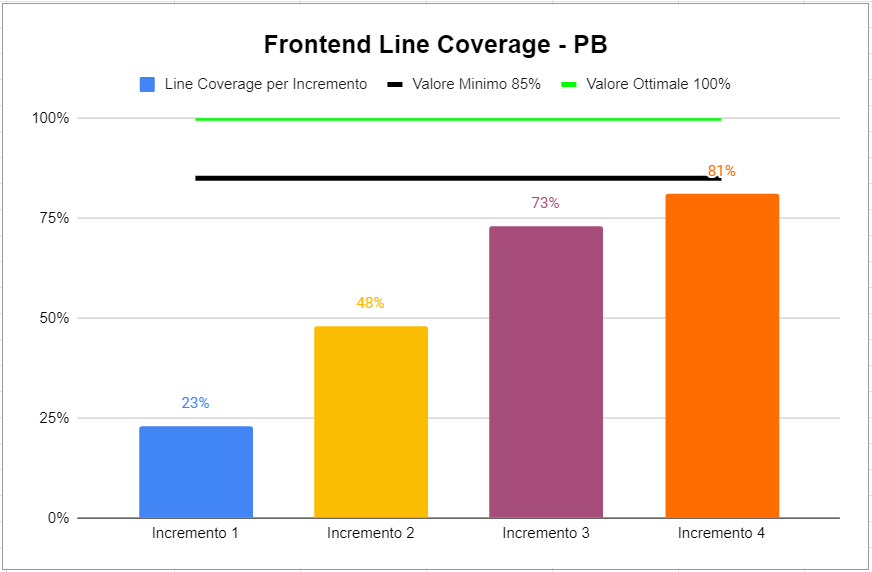
\includegraphics[width=0.8\textwidth, height=0.8\textheight,keepaspectratio]{images/PB-Frontend-Line.png}
  \caption{Grafico che rappresenta la matetrica di Line Coverage per la parte di Frontend nelle varie fasi della PB.}
\end{figure}    

\subsubsection{M20FBC - Frontend Branch Coverage}
\begin{figure}[H]
  \centering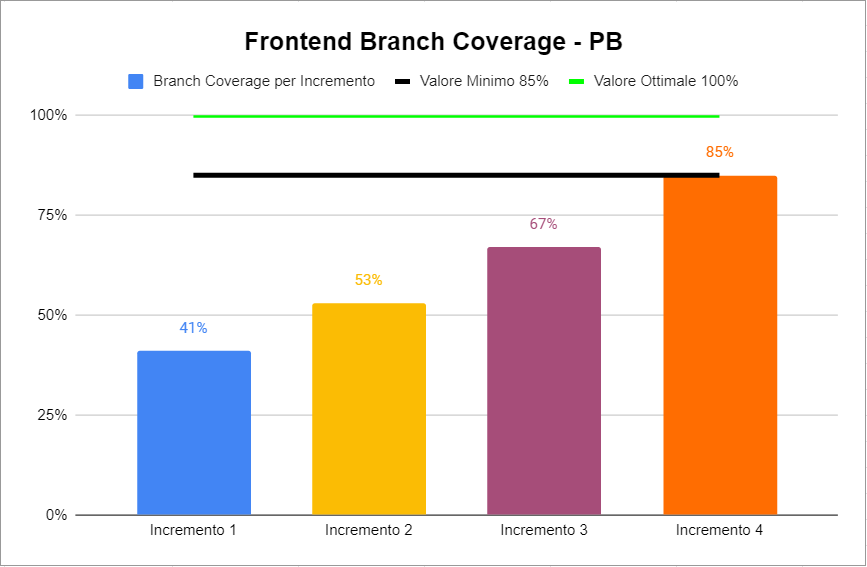
\includegraphics[width=0.8\textwidth, height=0.8\textheight,keepaspectratio]{images/PB-Frontend-Branch.png}
  \caption{Grafico che rappresenta la matetrica di Branch Coverage per la parte di Frontend nelle varie fasi della PB.}
\end{figure}    

\subsubsection{M21BLC - Backend Line Coverage}
\begin{figure}[H]
    \centering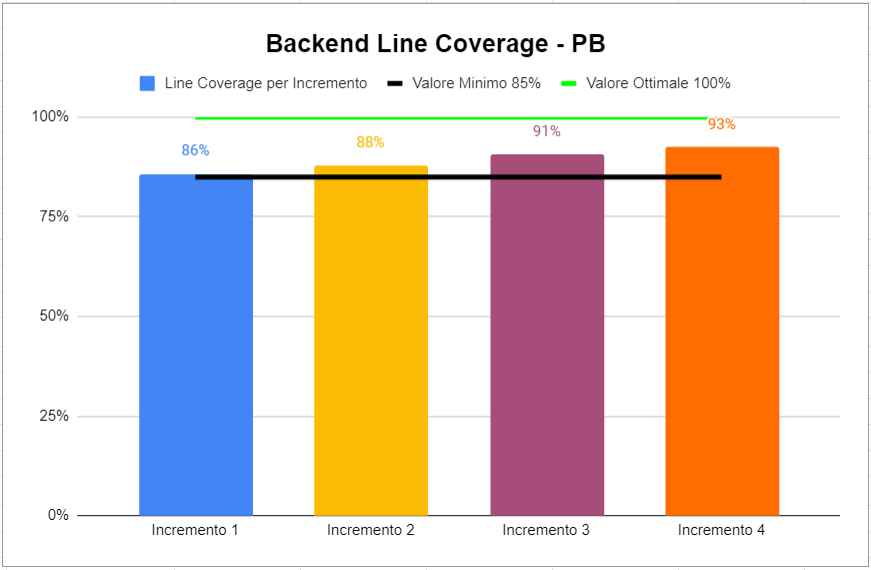
\includegraphics[width=0.8\textwidth, height=0.8\textheight,keepaspectratio]{images/PB-Backend-Line.png}
    \caption{Grafico che rappresenta la matetrica di Line Coverage per la parte di Backend nelle varie fasi della PB.}
\end{figure}    

\subsubsection{M22BBC - Backend Branch Coverage}
\begin{figure}[H]
  \centering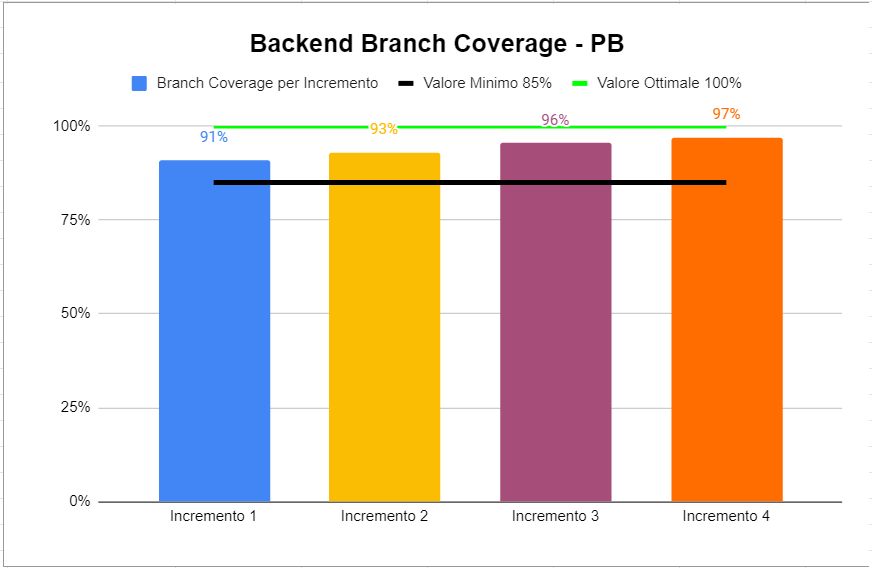
\includegraphics[width=0.8\textwidth, height=0.8\textheight,keepaspectratio]{images/PB-Backend-Branch.png}
  \caption{Grafico che rappresenta la matetrica di Branch Coverage per la parte di Backend nelle varie fasi della PB.}
\end{figure}    
 
\subsubsection{M23TPF - Test Passati Frontend}
Valore calcolato in base ai Test Eseguiti. Questi sono sempre risultati corretti alla fine di ogni incremento.
\begin{figure}[H]
  \centering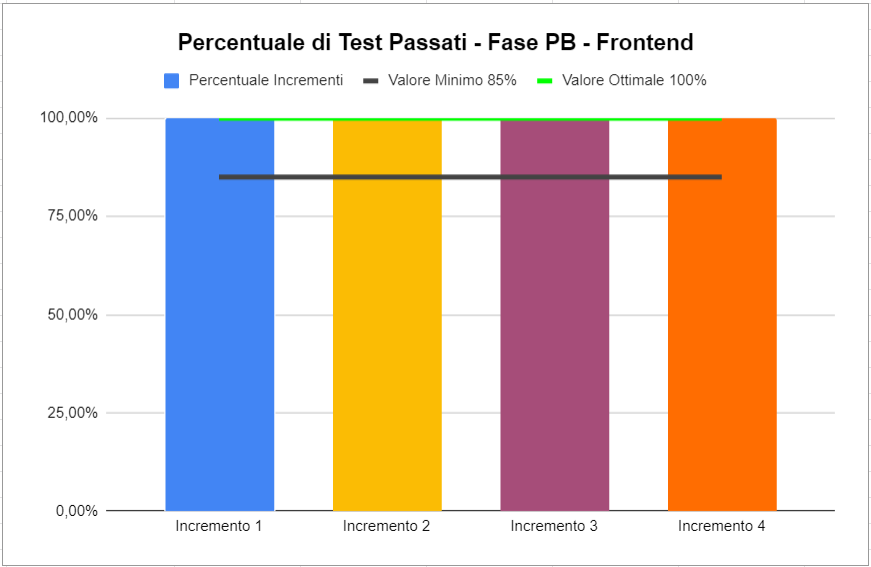
\includegraphics[width=0.7\textwidth, height=0.7\textheight,keepaspectratio]{images/PB-Test-Passati-Frontend.png}
  \caption{Grafico che rappresenta la percentuale di test passati per la parte di Frontend nelle varie fasi della PB.}
\end{figure}    

\subsubsection{M24TPB - Test Passati Backend}
Valore calcolato in base ai Test Eseguiti. Questi sono sempre risultati corretti alla fine di ogni incremento
\vspace{1em}
\begin{figure}[H]
  \centering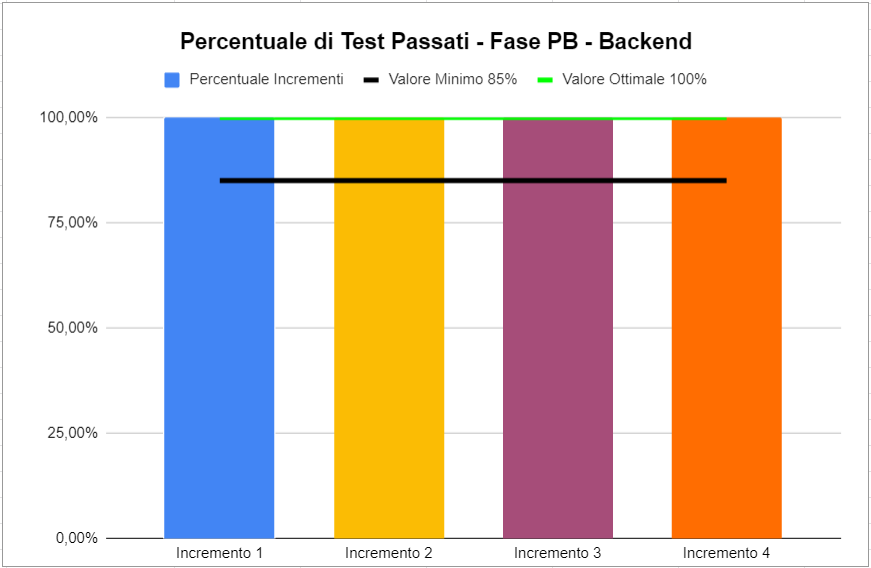
\includegraphics[width=0.7\textwidth, height=0.7\textheight,keepaspectratio]{images/PB-Test-Passati-Backend.png}
  \caption{Grafico che rappresenta la percentuale di test passati per la parte di Backend nelle varie fasi della PB.}
\end{figure}    



\subsection{Macrofase CA}

\subsubsection{M14IG - Indice di Gulpease}
\begin{figure}[H]
    \centering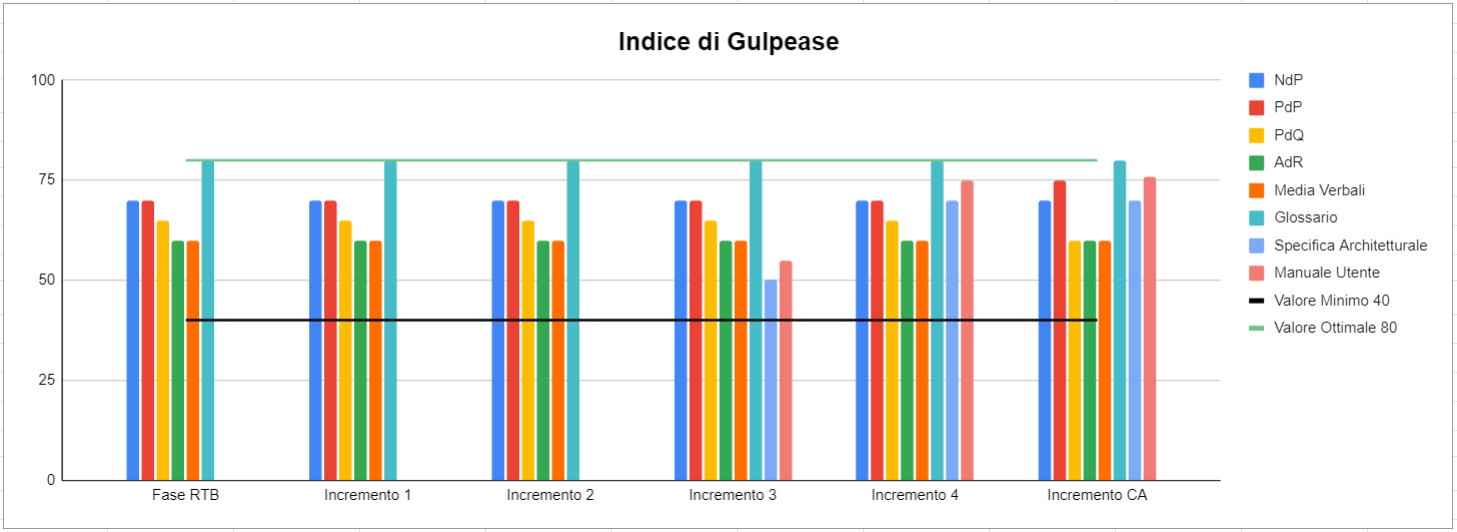
\includegraphics[width=\textwidth, height=\textheight,keepaspectratio]{images/CA-Indice-di-Gulpease.png}
    \caption{Grafico dell'indice di Gulpease dei documenti nelle varie fasi della PB.}
\end{figure}    

\subsubsection{M15VC - Variazione di Costo}
\begin{figure}[H]
    \centering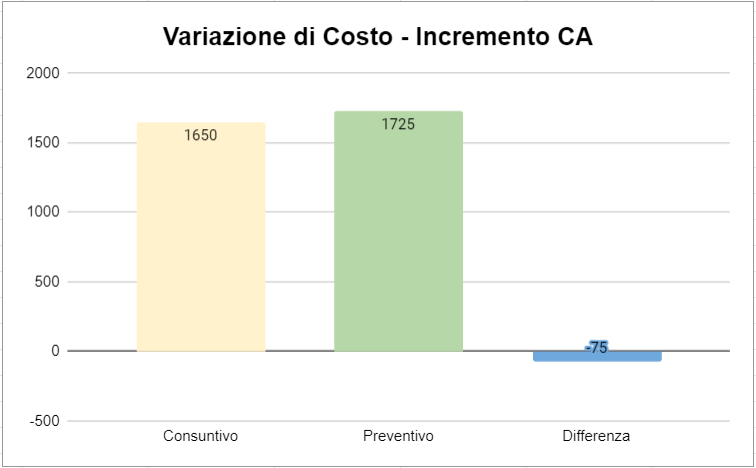
\includegraphics[width=0.8\textwidth, height=0.8\textheight,keepaspectratio]{images/CA-Variazione-di-Costo.png}
    \caption{Grafico che indica come sono variati i costi rispetto a quelli preventivati nelle varie fasi della PB.}
\end{figure}    

\subsubsection{M16VP - Variazione di Piano}
\begin{figure}[H]
   \centering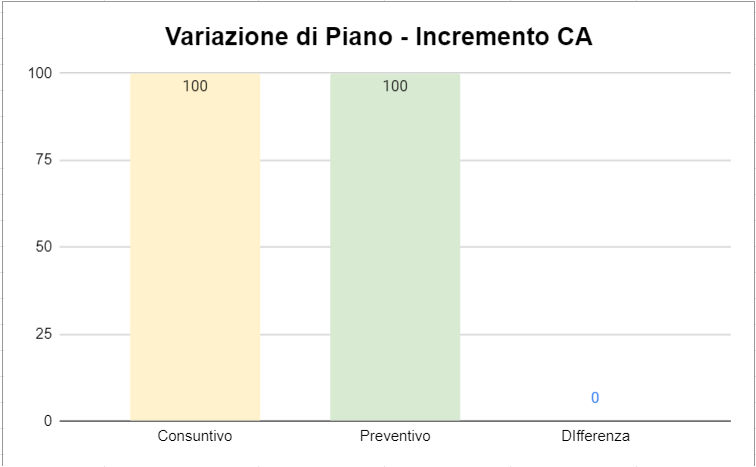
\includegraphics[width=0.8\textwidth, height=0.8\textheight,keepaspectratio]{images/CA-Variazione-di-Piano.png}
    \caption{Grafico che indica come è variata la pianificazione rispetto al preventivo nelle varie fasi della PB.}
\end{figure}  

\subsubsection{M8CC - Code Coverage}
Grafico di tipo Sunburst presente nel sito Codecov. \\
Il cerchio più interno rappresenta il progetto intero ed ogni cerchio esterno rappresenta una suddivisione in cartelle. \\
Ad ognuna viene associato un colore in base al coverage, da rosso se tendente allo 0\% a verde se tendente al 100\%.
\begin{figure}[H]
   \centering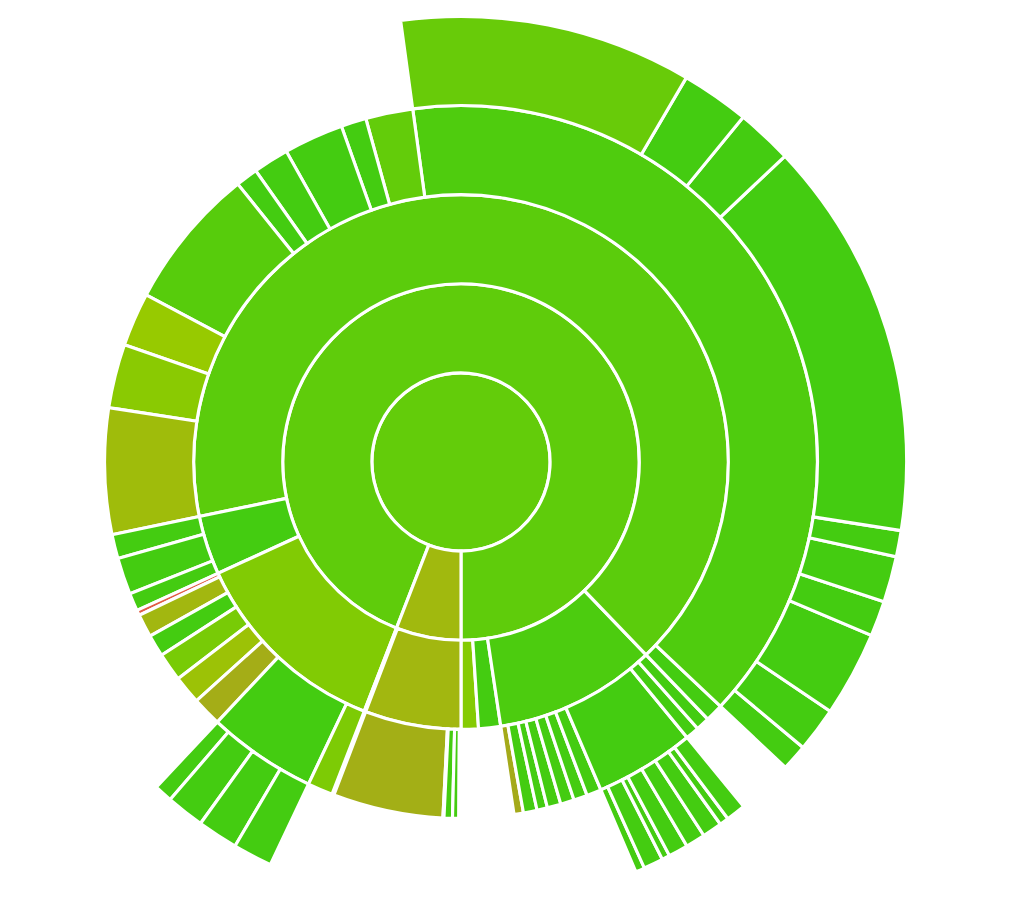
\includegraphics[width=0.5\textwidth, height=0.5\textheight,keepaspectratio]{images/graph.png}
    \caption{Grafico fornito da Codecov che mostra come ogni cartella del progetto sia stata testata.}
\end{figure}  

\begin{figure}[H]
  \centering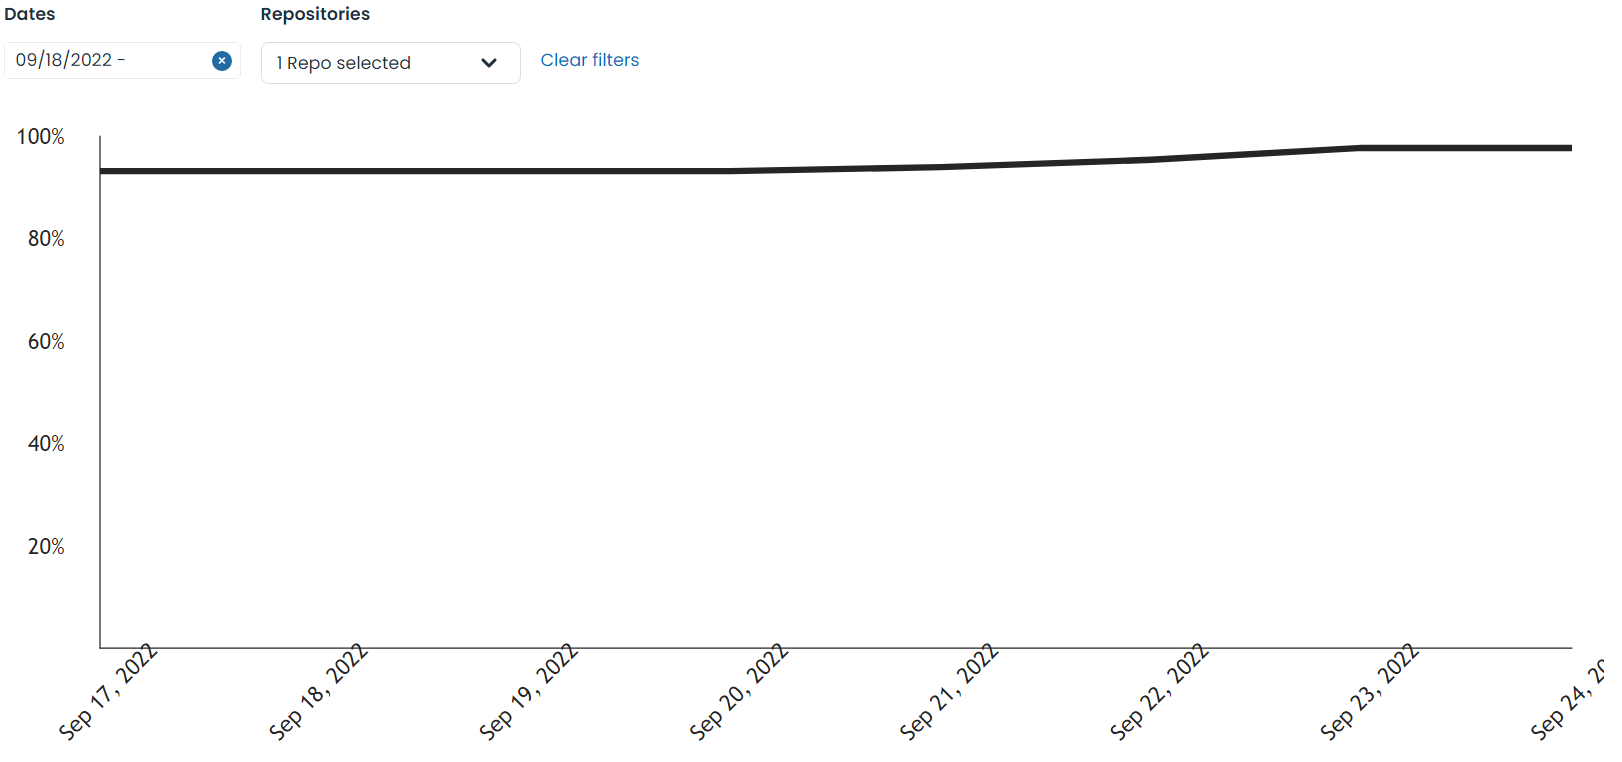
\includegraphics[width=0.9\textwidth, height=0.9\textheight,keepaspectratio]{images/CA-CodeCov.png}
   \caption{Grafico fornito da Codecov che mostra l'andamento di Code Coverage nella fase di CA.}
\end{figure}  

\subsubsection{M1PRR - Percentuale di Requisiti Obbligatori Soddisfatti}
\begin{figure}[H]
   \centering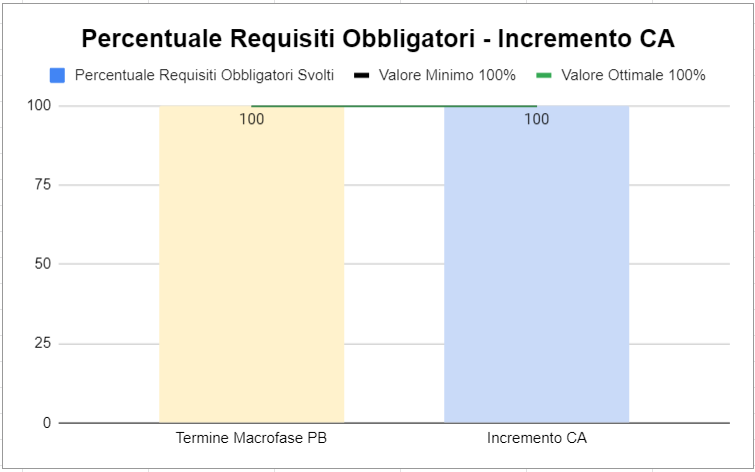
\includegraphics[width=0.8\textwidth, height=0.8\textheight,keepaspectratio]{images/CA-Requisiti-Obbligatori-Soddisfatti.png}
    \caption{Grafico che indica come è variata la percentuale di requisiti obbligatori soddisfatti.}
\end{figure}  
 
\subsubsection{M2PDR - Percentuale di Requisiti Desiderabili Soddisfatti}
\begin{figure}[H]
    \centering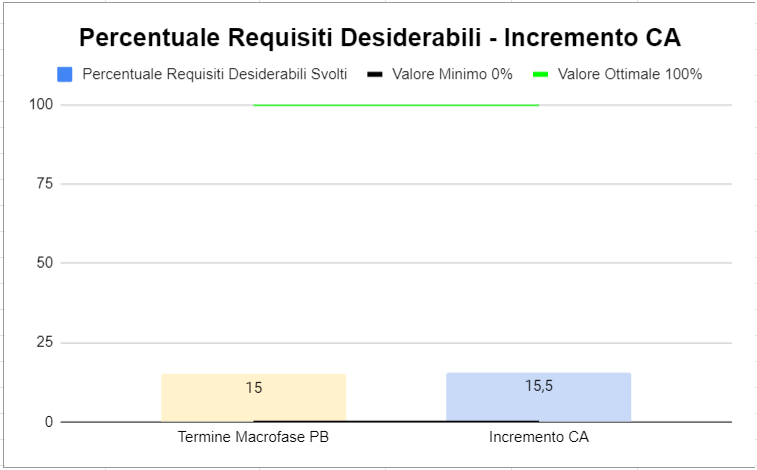
\includegraphics[width=0.8\textwidth, height=0.8\textheight,keepaspectratio]{images/CA-Requisiti-Desiderabili-Soddisfatti.png}
    \caption{Grafico che indica come è variata la percentuale di requisiti desiderabili soddisfatti.}
\end{figure}  

\subsubsection{M5ATC - Accoppiamento tra Classe}
\begin{figure}[H]
 \centering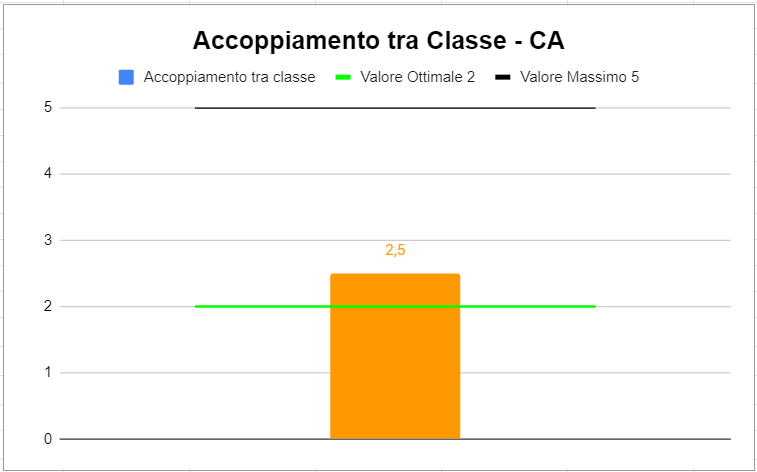
\includegraphics[width=0.8\textwidth, height=0.8\textheight,keepaspectratio]{images/CA-Accoppiamento.png}
  \caption{Grafico che indica il valore ottenuto di Accoppiamento tra le classi.}
\end{figure}  

\subsubsection{M6PDG - Profondità delle Gerarchie }
\begin{figure}[H]
 \centering\includegraphics[width=0.8\textwidth, height=0.8\textheight,keepaspectratio]{images/CA-Profondità.png}
  \caption{Grafico che indica il valore ottenuto di Profondità delle Gerarchie.}
\end{figure}  

\subsubsection{M9NAC - Numero di Attributi per Classe \& M10PF - Parametri per Funzione}
\begin{figure}[H]
 \centering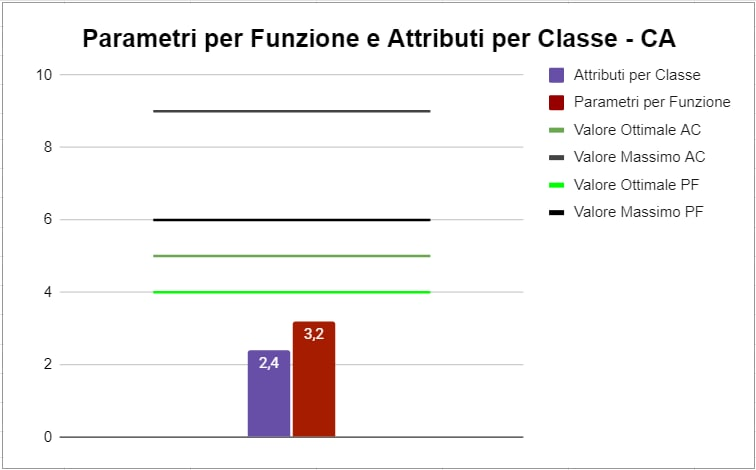
\includegraphics[width=0.8\textwidth, height=0.8\textheight,keepaspectratio]{images/CA-Parametri.png}
  \caption{Grafico che indica rispettivamente le medie dei valori di Attributi per classe e di Parametri per Funzione.}
\end{figure}  

\subsubsection{M13CPC - Linee di Commento per Linee di Codice}
\begin{figure}[H]
 \centering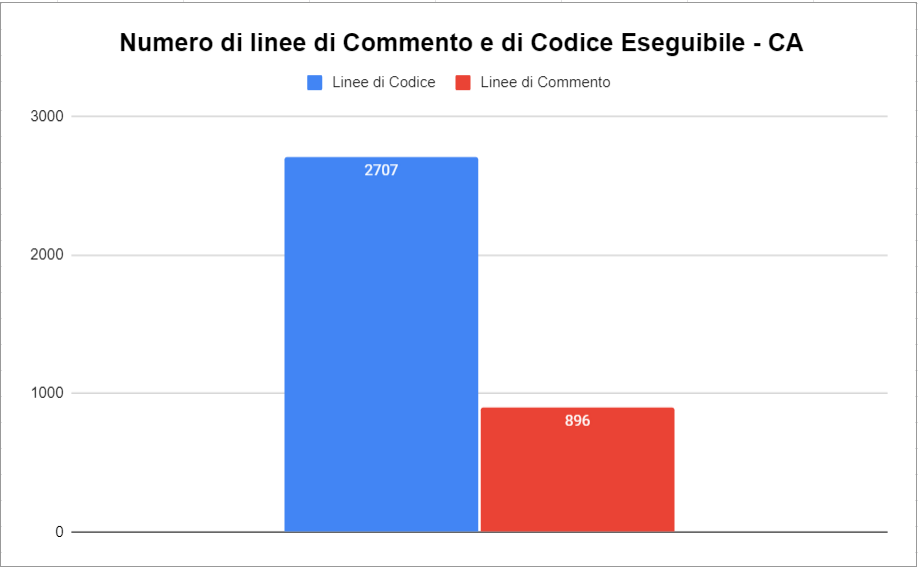
\includegraphics[width=0.8\textwidth, height=0.8\textheight,keepaspectratio]{images/CA-Commento.png}
  \caption{Grafico che mette a confronto il numero di righe di codice con il numero di righe di commento ad esso associate.}
\end{figure}  
\begin{figure}[H]
  \centering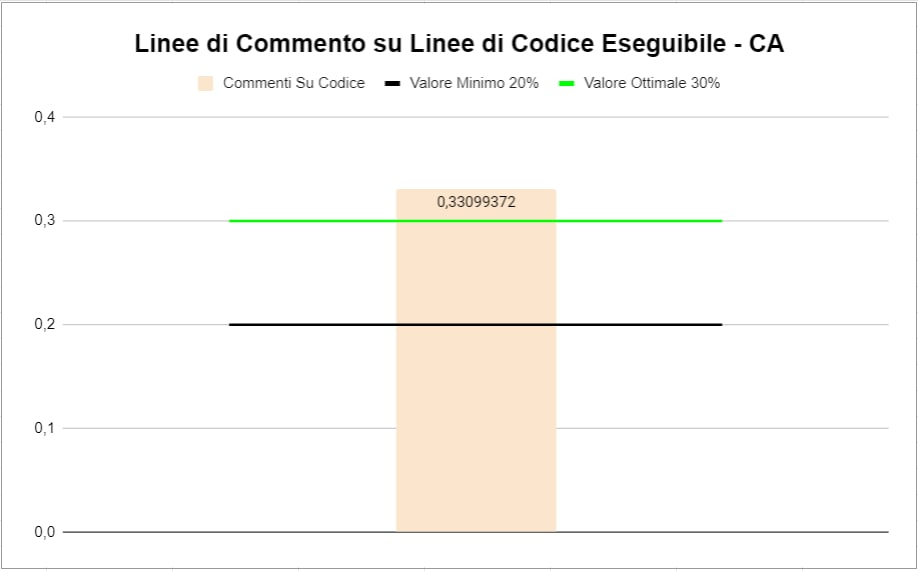
\includegraphics[width=0.8\textwidth, height=0.8\textheight,keepaspectratio]{images/CA-Commento-Codice.png}
   \caption{Grafico che mostra la metrica di linee di commento per linee di codice.}
 \end{figure}  

\subsubsection{M16FA - Facilità di Apprendimento}
 \begin{figure}[H]
  \centering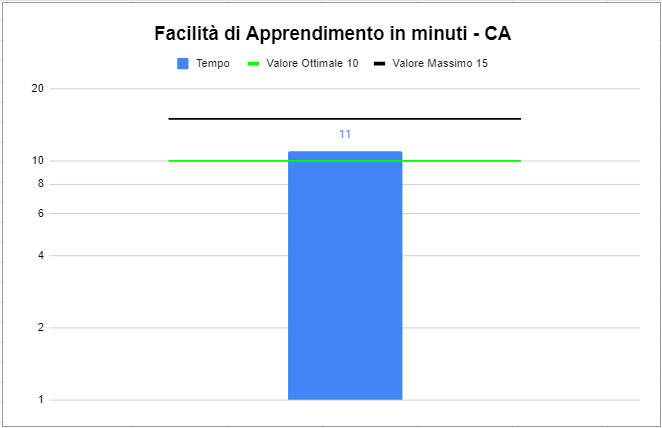
\includegraphics[width=0.8\textwidth, height=0.8\textheight,keepaspectratio]{images/CA-Apprendimento.png}
   \caption{Grafico che indica il tempo medio di Apprendimento necessari all'utilizzo dell'applicazione.}
 \end{figure} 

\subsubsection{M17EG - Errori Gestiti \& M18PM - Percentuale Malfunzionamenti}
\begin{figure}[H]
 \centering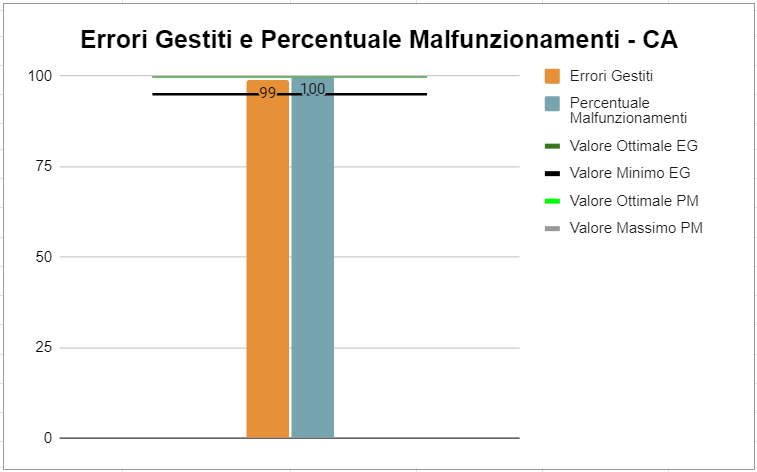
\includegraphics[width=0.8\textwidth, height=0.8\textheight,keepaspectratio]{images/CA-Errori.png}
  \caption{Grafico che indica rispettivamente la percentuale di errori gestiti e la percentuale di Malfunzionamenti gestiti.}
\end{figure}  

\subsubsection{M19FLC - Frontend Line Coverage}
\begin{figure}[H]
 \centering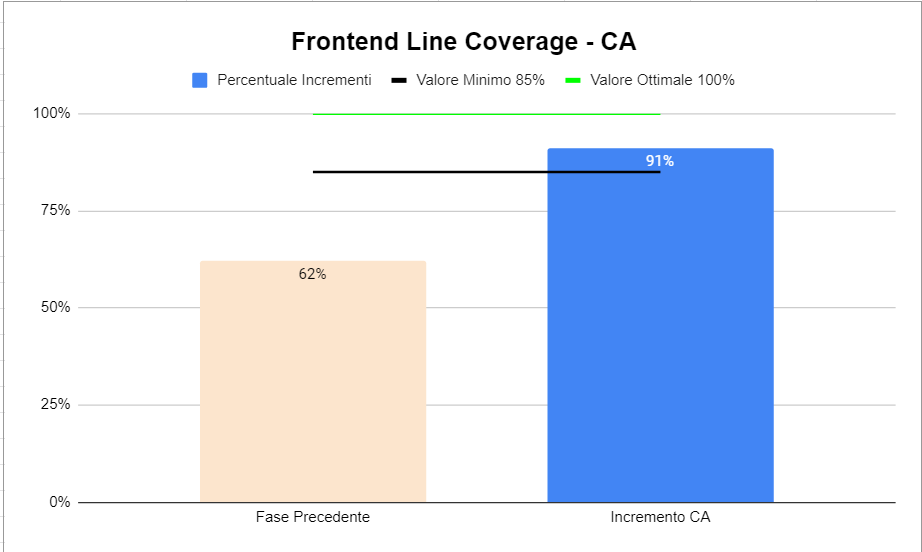
\includegraphics[width=0.6\textwidth, height=0.6\textheight,keepaspectratio]{images/CA-Frontend-Line.png}
  \caption{Grafico che rappresenta la matetrica di Line Coverage per la parte di Frontend nell'unico incremento della fase CA}
\end{figure}    

\subsubsection{M20FBC - Frontend Branch Coverage}
\begin{figure}[H]
  \centering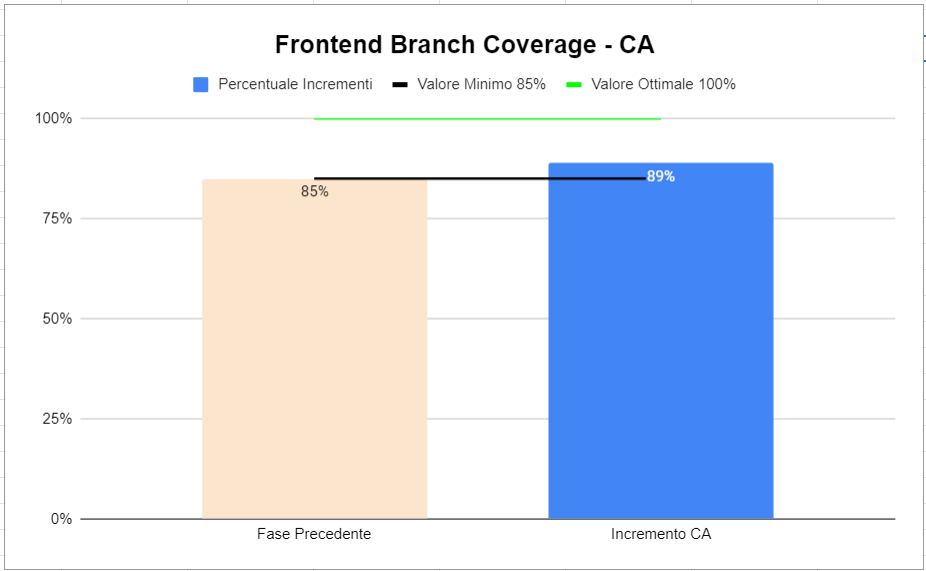
\includegraphics[width=0.6\textwidth, height=0.6\textheight,keepaspectratio]{images/CA-Frontend-Branch.png}
  \caption{Grafico che rappresenta la matetrica di Branch Coverage per la parte di Frontend nell'unico incremento della fase CA.}
\end{figure}    

\subsubsection{M21BLC - Backend Line Coverage}
\begin{figure}[H]
    \centering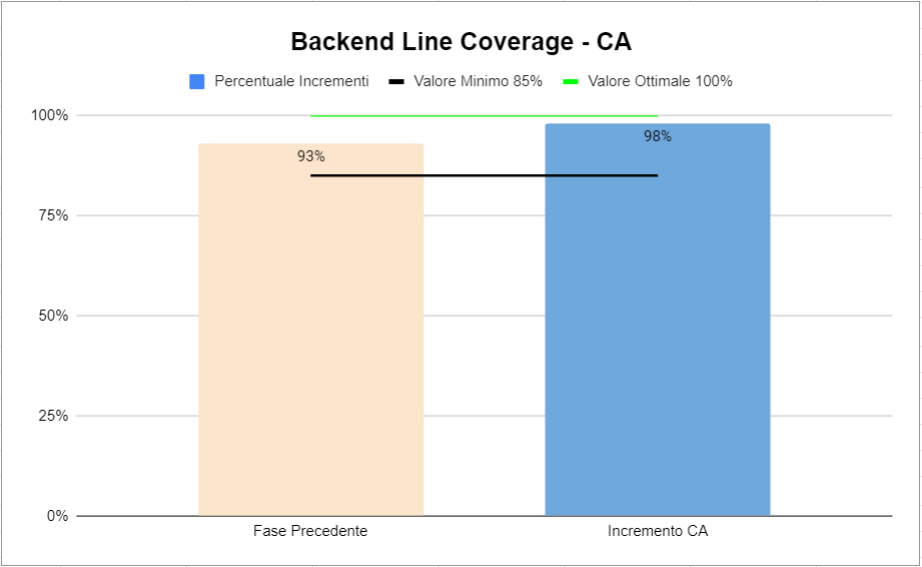
\includegraphics[width=0.6\textwidth, height=0.6\textheight,keepaspectratio]{images/CA-Backend-Line.png}
    \caption{Grafico che rappresenta la matetrica di Line Coverage per la parte di Backend nell'unico incremento della fase CA}
\end{figure}    

\subsubsection{M22BBC - Backend Branch Coverage}
\begin{figure}[H]
  \centering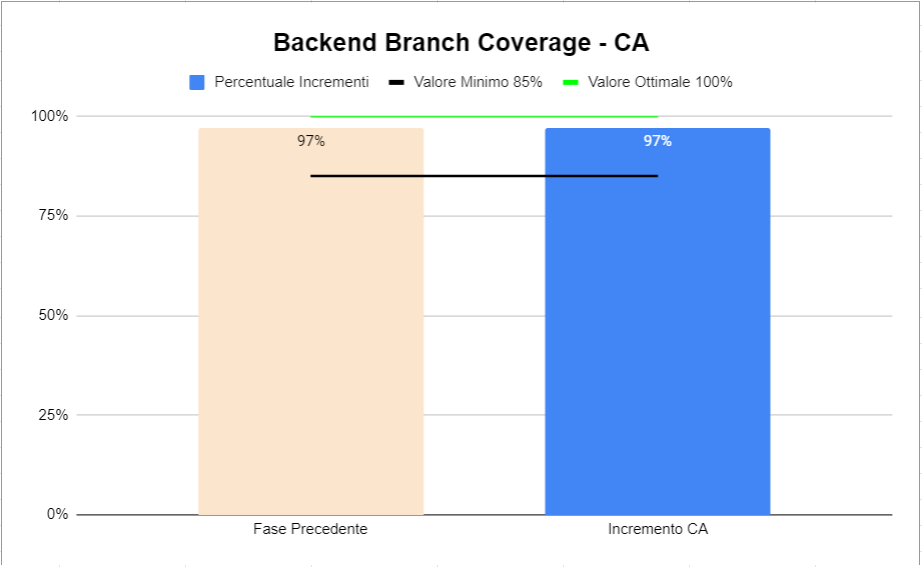
\includegraphics[width=0.6\textwidth, height=0.6\textheight,keepaspectratio]{images/CA-Backend-Branch.png}
  \caption{Grafico che rappresenta la matetrica di Branch Coverage per la parte di Backend nell'unico incremento della fase CA}
\end{figure}    

\subsubsection{M23TPF - Test Passati Frontend}  
\begin{figure}[H]
  \centering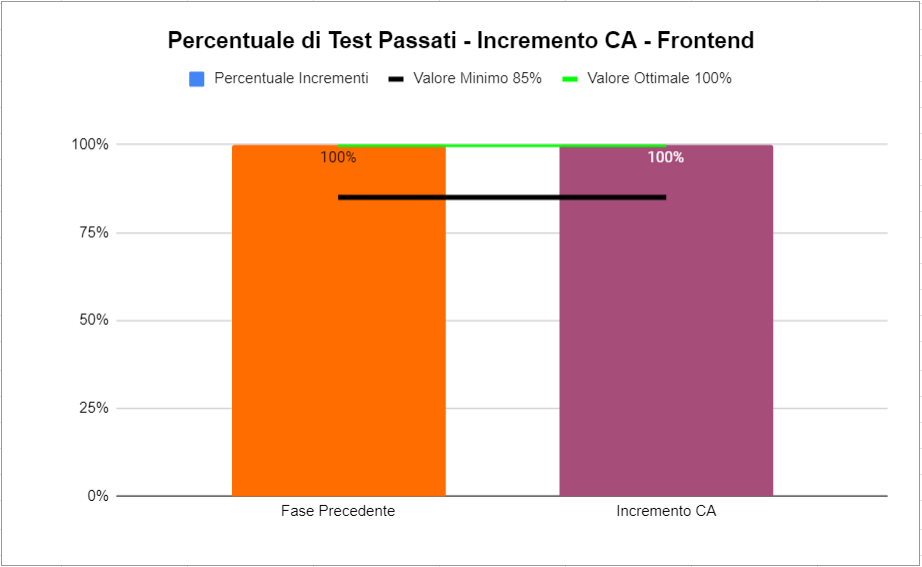
\includegraphics[width=0.6\textwidth, height=0.6\textheight,keepaspectratio]{images/CA-Test-Passati-Frontend.png}
  \caption{Grafico che rappresenta la percentuale di test passati per la parte di Frontend nell'unico incremento della fase CA}
\end{figure}    

\subsubsection{M24TPB - Test Passati Backend}
\begin{figure}[H]
  \centering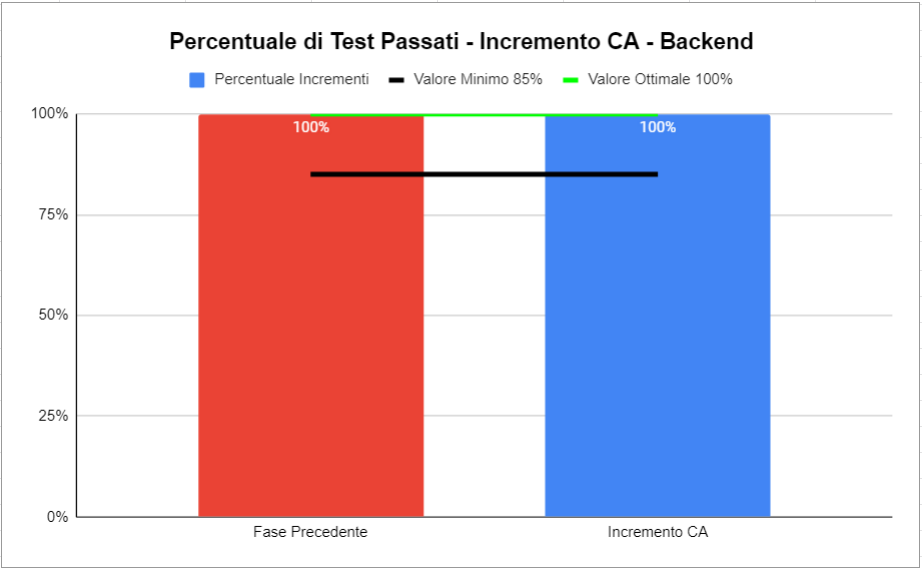
\includegraphics[width=0.6\textwidth, height=0.6\textheight,keepaspectratio]{images/CA-Test-Passati-Backend.png}
  \caption{Grafico che rappresenta la percentuale di test passati per la parte di Backend nell'unico incremento della fase CA.}
\end{figure}    